\chapter{ Refonte de la chaîne Data et décisionnelle d'IPANEMA Introduction  }
\minitoc
\label{chap1}
\newpage
%=====================================%
\section{Introduction}
\label{sec11}
%=====================================% 
Ce rapport d'action présente une synthèse du projet IPANEMA mené au cours de mon 
alternance au sein de la R&D Dermo-Cosmétique & Personal Care de Pierre Fabre. Il expose 
le problème à l'origine du projet, les objectifs fixés, la réponse apportée, les résultats obtenus 
à ce stade ainsi que les principaux éléments ayant permis son pilotage. Il vise ainsi à donner 
une vision globale du travail réalisé et de sa contribution au suivi des Tierces Parties par les 
équipes Qualité.
%=====================================%


\section{Contexte et problématique}
\label{sec13}
%=====================================%
IPANEMA (International Partners Network & Management) est une solution 
informatique utilisée dans le cadre du processus de maîtrise des Tierces Parties de la R&D 
DC&PC. Elle accompagne notamment l'évaluation et le suivi d'entités extérieures dont les 
activités peuvent avoir un impact direct ou indirect sur la qualité d'un produit ou sur la sécurité 
du patient, du consommateur ou du client. La pertinence de ce suivi repose donc en partie sur 
la fiabilité des données collectées, traitées et restituées. 

Le projet IPANEMA v2 comporte deux périmètres complémentaires. La refonte de 
l'application métier sous Power Apps (dite Partie A) a été confiée à un prestataire externe. 
Mon projet correspond à la Partie B du cahier des charges : la refonte de la chaîne Data et du 
reporting associé, c'est-à-dire la partie décisionnelle d'IPANEMA. Démarré en février 2026, ce 
projet s'est déroulé en suivant la stabilisation de la Partie A. En tant que Data Analyst, j'ai pris 
en charge ce périmètre dans son ensemble, depuis l'analyse de l'existant et du besoin jusqu'au 
développement de la nouvelle solution de restitution. 

Dans l'architecture historique, les données saisies dans IPANEMA étaient réparties 
dans plusieurs listes SharePoint. Elles étaient ensuite préparées à l'aide d'Alteryx. Le workflow 
existant les consolidait dans une table unique destinée à alimenter un dashboard Tableau. 
L'analyse de cette chaîne a cependant mis en évidence plusieurs limites : certaines opérations 
de jointure pouvaient entraîner des duplications ou des pertes d'enregistrements, avec des 
répercussions sur la restitution de certains indicateurs. 

Ces difficultés étaient notamment liées à la structure même des données. Les 
informations manipulées ne présentent pas toutes le même niveau de détail : une Tierce Partie 
peut, par exemple, être associée à plusieurs campagnes et plusieurs évaluations. La 
consolidation de ces informations dans une seule table pouvait donc altérer leur structure et 
complexifier leur exploitation.

À cette problématique de fiabilité s'ajoutait un enjeu de pérennité. L'environnement 
décisionnel du groupe évoluant vers Power BI et l'écosystème Microsoft, le projet représentait 
l'opportunité de ne pas simplement reproduire le dashboard existant dans un nouvel outil, mais 
de repenser la chaîne de valorisation de la donnée dans son ensemble.

Cette problématique, déjà énoncée en introduction générale, structure l'ensemble du 
rapport d'action qui suit. 

\section{Objectifs et critères d'évaluation}

\label{sec12}
 %=====================================%
Le diagnostic de l'existant et les échanges avec les parties prenantes ont permis de 
structurer le projet autour de trois enjeux principaux — fiabiliser la donnée, faciliter son 
exploitation et assurer la pérennité de la solution — déclinés en cinq objectifs opérationnels 
associés à des critères d'évaluation concrets. 

Afin de ne pas limiter ces objectifs à des intentions générales, des critères permettant d'apprécier leur atteinte ont également été identifiés, conformément à une logique de validation progressive puis de recette utilisateurs

\begin{table}[h!]
\centering
\caption{Objectifs et critères d'évaluation du projet IPANEMA}
\label{tab:objectifs-criteres}
\vspace{6pt}
\renewcommand{\arraystretch}{1.5} % Augmente l'espace haut/bas dans les cellules
\setlength{\tabcolsep}{10pt}     % Augmente l'espace gauche/droite dans les cellules
\begin{tabular}{|>{\raggedright\arraybackslash}p{5cm}|>{\raggedright\arraybackslash}p{8.5cm}|}
\hline
\textbf{Objectif} & \textbf{Critère d'évaluation} \\
\hline
Fiabiliser les données et les indicateurs & Cohérence des données restituées et conformité des indicateurs avec les règles métier \\
\hline
Repenser la structuration des données & Respect des différents niveaux de détail et de leurs relations \\
\hline
Améliorer la restitution de l'information & Lisibilité et adéquation du dashboard avec les besoins des équipes Qualité \\
\hline
Faciliter la maintenance et les évolutions & Séparation et documentation plus claires des différentes étapes de traitement \\
\hline
Accompagner l'évolution du SI & Mise à disposition du reporting sous Power BI \\
\hline
\end{tabular}
\end{table}

Ces objectifs traduisent la double dimension du projet. Il ne s'agissait pas uniquement 
de développer un nouveau dashboard, mais de sécuriser la donnée sur laquelle repose le 
pilotage, puis de proposer une restitution adaptée aux besoins des équipes Qualité. 

\section{Réponse apportée}
\label{sec121}
L'analyse de l'existant a montré qu'une simple migration du dashboard Tableau vers 
Power BI aurait conservé une partie des difficultés déjà identifiées. La réponse apportée a 
donc consisté à intervenir à la fois sur l'organisation des données en amont et leur restitution 
en aval. 

J'ai ainsi retravaillé la préparation des données sous Alteryx afin de ne plus produire 
une unique table à plat, mais plusieurs ensembles de données structurés selon leur niveau de 
détail. Sur cette nouvelle base, j'ai construit le modèle nécessaire à leur exploitation dans 
Power BI. J'ai ensuite développé les indicateurs attendus et réalisé le nouveau dashboard 
destiné aux équipes Qualité. Le travail effectué sur Alteryx permet notamment de conserver 
séparément les données de granularités différentes. Il limite également les jointures globales 
à l'origine de certaines incohérences de l'ancienne solution.

La réponse mise en œuvre peut être représentée synthétiquement de la manière 
suivante :

\begin{figure}[h!]
\centering
\begin{tcolorbox}[
    colframe=gray!60,       % Couleur de la bordure (gris léger)
    colback=white,          % Couleur de fond
    boxrule=0.8pt,          % Épaisseur du cadre
    arc=3pt,                % Arrondi des angles
    boxsep=4pt,             % Espacement interne global
    left=4pt, right=4pt, top=4pt, bottom=4pt
]
    \centering
    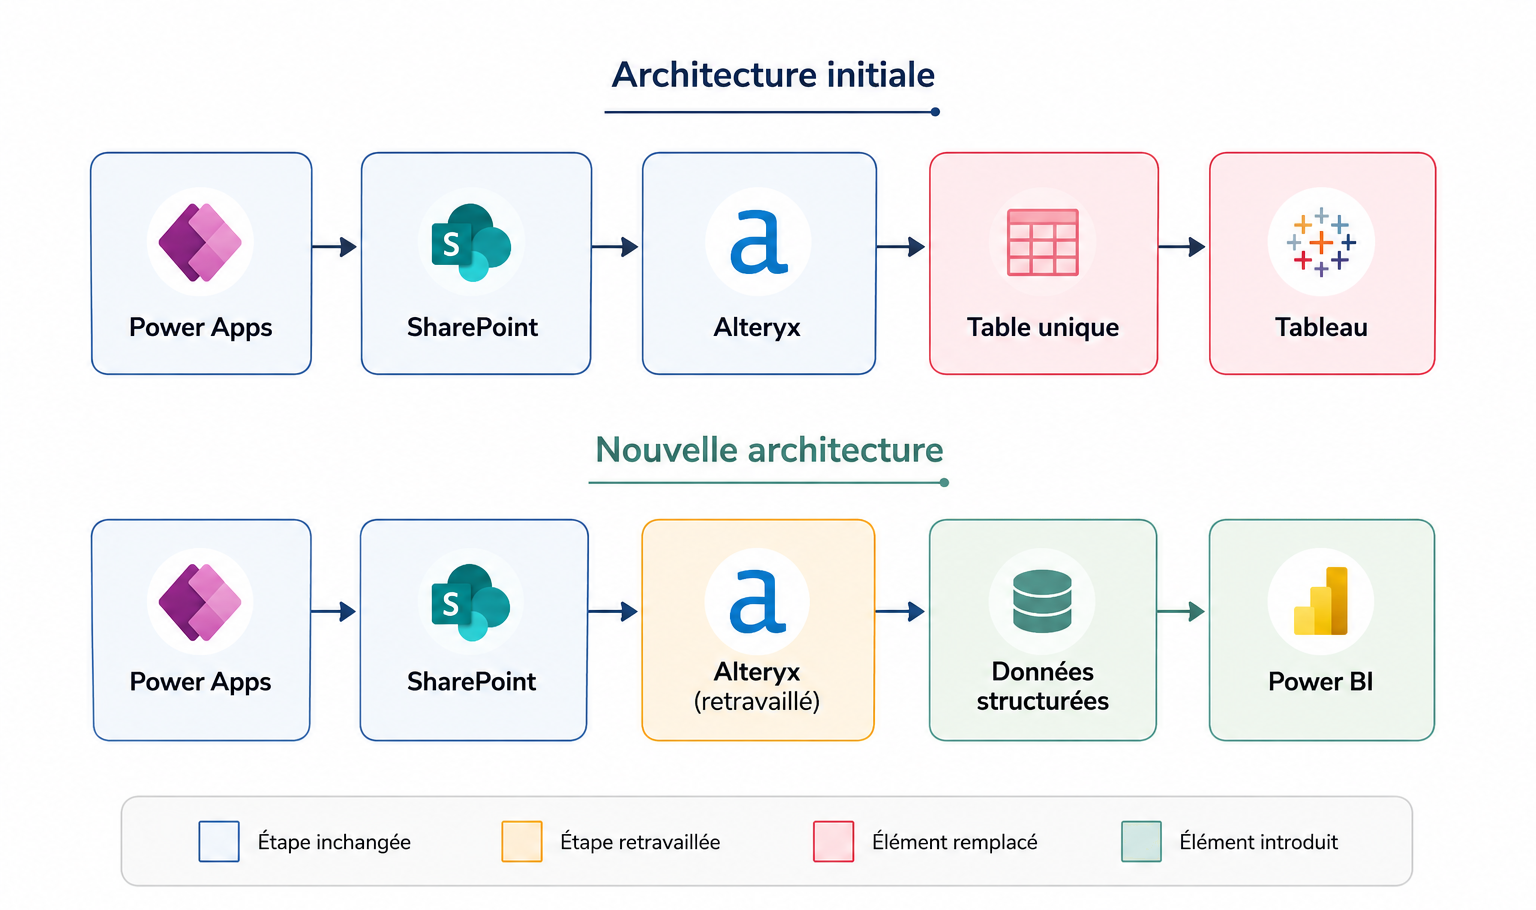
\includegraphics[draft=false,width=\textwidth]{cover/figures/archii_avant_apres.png}
\end{tcolorbox}
\caption{Évolution synthétique de la chaîne Data et décisionnelle d'IPANEMA}
\label{fig:evolution-architecture-ipanema}
\end{figure}

Le changement réalisé ne se résume donc pas au remplacement de Tableau par Power 
BI. Il repose également sur une refonte de la manière dont les données sont préparées et 
organisées avant leur restitution. Les choix de modélisation, les traitements réalisés et les 
aspects techniques de cette architecture seront développés dans le rapport d'étude.

\section{Réalisations et résultats obtenus}

Sur la base de cette réponse technique, les travaux ont été conduits jusqu'à leur terme 
selon la démarche itérative présentée en 1.5. À la date de rédaction de ce mémoire, le 
développement de la nouvelle solution est arrivé à son terme sur le plan fonctionnel et 
technique, la solution étant fonctionnelle de bout en bout. Mon intervention a couvert l'analyse 
de la chaîne existante, l'identification de ses limites, la restructuration des traitements de 
données, la construction du nouveau modèle, le développement des indicateurs et la 
réalisation du dashboard Power BI.

Ces travaux ont permis de faire évoluer IPANEMA d'une logique reposant sur une table 
unique vers une organisation structurée selon les différents niveaux de détail des données. La 
préparation, la structuration, les calculs et la restitution sont désormais davantage distingués, 
ce qui vise à rendre la chaîne plus compréhensible et plus facilement maintenable.

Le projet aboutit également à un nouveau dashboard développé sous Power BI, permettant d'inscrire le reporting IPANEMA dans l'environnement décisionnel cible. La solution 
obtenue répond ainsi à la fois à l'enjeu initial de fiabilisation de la donnée et à l'objectif de 
migration technologique.

\begin{table}[h!]
\centering
\caption{Comparaison avant/après le projet IPANEMA}
\label{tab:avant-apres-ipanema}
\vspace{6pt}
\renewcommand{\arraystretch}{1.5} % Augmente l'espace haut/bas dans les cellules
\setlength{\tabcolsep}{10pt}     % Augmente l'espace gauche/droite
\begin{tabular}{|>{\raggedright\arraybackslash}p{5cm}|>{\raggedright\arraybackslash}p{8.5cm}|}
\hline
\textbf{Avant le projet} & \textbf{À l'issue du développement} \\
\hline
Consolidation dans une table unique & Données organisées selon leurs différents niveaux de détail \\
\hline
Jointures pouvant générer des duplications ou pertes d'enregistrements & Restructuration des traitements afin de limiter ces situations \\
\hline
Reporting sous Tableau & Nouveau reporting développé sous Power BI \\
\hline
Chaîne complexe à faire évoluer & Séparation plus claire des différentes étapes de traitement \\
\hline
Contrôle principalement sur le résultat final & Tests et ajustements progressifs au cours du développement \\
\hline
\end{tabular}
\end{table}

La validation n'a pas été reportée à la seule fin du projet. Des tests et des revues ont 
été réalisés progressivement pendant le développement avec l'interlocuteur métier impliqué 
dans son suivi. Ces échanges ont permis de confronter régulièrement les réalisations au 
besoin, d'identifier les écarts et d'apporter les ajustements nécessaires. Les retours obtenus à 
ce stade sont favorables et confortent les orientations retenues.

La dernière étape avant la mise en production reste néanmoins la recette fonctionnelle 
élargie aux différents utilisateurs d'IPANEMA. Son organisation a été décalée en raison de 
contraintes de calendrier et de disponibilité des parties prenantes, notamment pendant la 
période estivale. 

Cette recette sera organisée sous la forme de demi-journées d'ateliers dédiés. Des 
scénarios représentatifs des usages d'IPANEMA seront définis puis exécutés avec les 
différents profils utilisateurs afin de vérifier la cohérence des données, la conformité des 
indicateurs et l'adéquation du dashboard avec les usages métier. Les retours recueillis 
permettront de distinguer les éventuelles anomalies devant être corrigées avant la mise en 
production des demandes d'amélioration susceptibles d'alimenter une évolution ultérieure de 
la solution. 

À ce stade, le bilan doit donc être nuancé : les objectifs liés à la restructuration de la 
chaîne Data et au développement sous Power BI sont atteints sur le plan de la réalisation, 
tandis que la validation définitive de certains critères fonctionnels reste conditionnée aux 
ateliers de recette. Cette distinction permet de ne pas considérer comme définitivement validés 
des résultats qui doivent encore être confrontés à l'ensemble des utilisateurs. 

\section{Principaux éléments de management du projet}

Le projet IPANEMA a été conduit selon une démarche agile adaptée au fonctionnement 
de l'équipe, fondée sur des cycles courts de réalisation, de validation et d'ajustement. Sans 
appliquer strictement un framework tel que Scrum, l'organisation retenue privilégie la 
collaboration, le feedback régulier et la capacité à adapter les travaux aux constats effectués 
au cours du projet.

Le pilotage s'appuie sur un suivi visuel des activités inspiré du Kanban, complété par 
des cartes mentales évolutives permettant de structurer les travaux et de capitaliser 
progressivement les informations nécessaires à leur documentation. Des points réguliers avec 
mon maître d'apprentissage permettent de partager l'avancement, de valider les orientations 
et de définir les prochaines étapes. Entre ces échanges, je conduis mes travaux de manière autonome et sollicite directement les personnes concernées lorsqu'un blocage nécessite un 
échange ou un arbitrage. 

La démarche peut ainsi être synthétisée par la boucle suivante :

\begin{center}
\begin{tcolorbox}[
    colframe=gray!60,       % Bordure gris doux
    colback=gray!4!white,   % Fond très clair
    boxrule=0.8pt,          % Épaisseur du cadre
    arc=5pt,                % Coins légèrement arrondis
    width=\textwidth,       % S'adapte à la largeur du texte
    halign=center,          % Centrage parfait du contenu
    top=8pt, bottom=8pt
]
\small\bfseries
Planifier 
\;\textcolor{gray!80}{$\longrightarrow$}\; 
Réaliser 
\;\textcolor{gray!80}{$\longrightarrow$}\; 
Tester 
\;\textcolor{gray!80}{$\longrightarrow$}\; 
Recueillir les retours 
\;\textcolor{gray!80}{$\longrightarrow$}\; 
Ajuster
\end{tcolorbox}
\end{center}


Cette logique s'est concrétisée par les validations progressives réalisées pendant le 
développement et se poursuivra lors des ateliers de recette. Elle permet de faire évoluer la 
solution en fonction des constats et des retours métier plutôt que d'attendre la fin du projet 
pour confronter le résultat aux besoins des utilisateurs. 

Cette présentation est volontairement synthétique. L'organisation des tâches, le 
schéma heuristique, les outils de pilotage, le planning prévisionnel et réalisé, l'analyse des 
écarts ainsi que les relations avec le maître d'apprentissage et l'équipe projet seront 
développés dans la partie spécifiquement consacrée au management du projet, conformément 
aux attendus de l'école.


\section{ Conclusion}
\label{sec16}
%=====================================%
Le projet IPANEMA a dépassé l'objectif initial d'une simple migration du reporting de 
Tableau vers Power BI. L'analyse de l'existant a mis en évidence la nécessité d'intervenir en 
amont de la visualisation afin de repenser la structuration des données et de fiabiliser leur 
exploitation. Le projet a ainsi abouti à une nouvelle chaîne Data structurée et à un nouveau 
dashboard Power BI destiné aux équipes Qualité. 

À ce stade, la réalisation technique est aboutie et la solution, fonctionnelle de bout en bout, a 
fait l'objet de validations progressives tout au long de son développement. Les ateliers de 
recette permettront désormais d'élargir cette validation aux différents utilisateurs avant la mise 
en production et, le cas échéant, d'identifier des améliorations pour une version ultérieure. Le 
rapport d'étude développera les analyses et les choix techniques ayant conduit à cette 
solution.
